% 固定来源PDF第2页第10题：正方体与过 B,D,C_1 的截面。
% u/v/w 只是立方体的平行投影基向量，不表示题设给出坐标或边长。
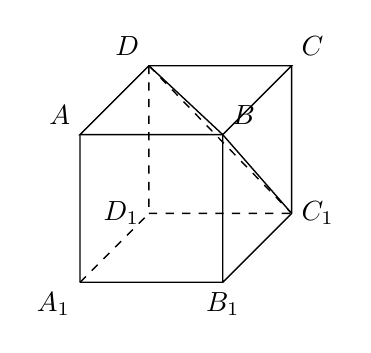
\begin{tikzpicture}[line width=.5pt,scale=1.25]
  \coordinate (A) at (0,1.7);
  \coordinate (B) at (1.45,1.7);
  \coordinate (C) at (2.15,2.4);
  \coordinate (D) at (.7,2.4);
  \coordinate (A1) at (0,.2);
  \coordinate (B1) at (1.45,.2);
  \coordinate (C1) at (2.15,.9);
  \coordinate (D1) at (.7,.9);
  % 可见外棱与隐藏外棱。
  \draw (A)--(B)--(C)--(D)--cycle;
  \draw (A)--(A1) (B)--(B1) (C)--(C1) (A1)--(B1)--(C1);
  \draw[dashed] (D)--(D1) (A1)--(D1) (D1)--(C1);
  % 截面 BDC_1：D C_1 位于背面，按投影用虚线表示。
  \draw (B)--(D) (B)--(C1);
  \draw[dashed] (D)--(C1);
  \node[above left] at (A) {$A$};
  \node[above right] at (B) {$B$};
  \node[above right] at (C) {$C$};
  \node[above left] at (D) {$D$};
  \node[below left] at (A1) {$A_1$};
  \node[below] at (B1) {$B_1$};
  \node[right] at (C1) {$C_1$};
  \node[left] at (D1) {$D_1$};
\end{tikzpicture}
